\chapter{Conclusiones y Líneas de trabajo futuras}

\section{Aprendizaje}
Este proyecto me ha servido mucho para profundizar en como funcionan los lenguajes de programación, los compiladores, los debuggers, etc.\\
En base a esto también he aprendido como funcionan asistentes como Spyder o Eclipse a la hora de marcar con colorines las palabras clave.\\
De forma similar al anterior los editores de texto como Word o Writer para notificarte faltas de ortografía y de construcción de frases.\\
En resumidas cuentas, me quedaron pendientes algunos conceptos de la asignatura de procesadores del lenguaje y este TFG ha sido muy útil para reforzarlos.

También me ha servido para establecerme metodologías de trabajo, horarios y fechas, establecer tareas para hacer un día o semana y por extensión también he aprendido a manejar la frustración a la hora de trabajar y la importancia de los descansos.

He aprendido como de distinto funcionan los punteros en C y Python, se profundizará en el tema cuando hable de las limitaciones de la herramienta.

\section{Limitaciones de la herramienta}
Por como están hechos los punteros en python y c, a pesar de que Python este implementado en C, no se puede adaptar el depurador a ellos ver \ref{fig:punteros1} y \ref{fig:punteros2}.
En Python los tipos primitivos cambian de posición en memoria cada vez que son editados.
\begin{figure}[ht]
\centering
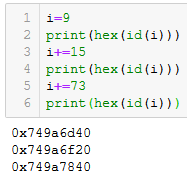
\includegraphics[width=0.4\textwidth]{img/punterosP1.png}
\caption{Ejemplo de un puntero en Python}
\label{fig:punteros1}
\end{figure}
\begin{figure}[ht]
\centering
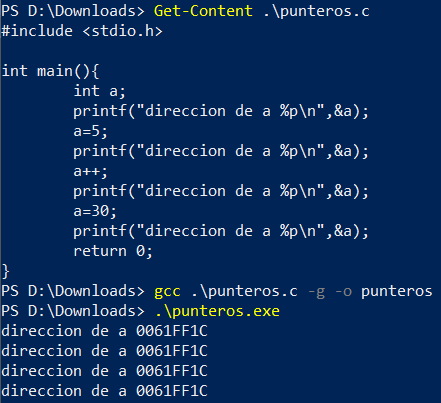
\includegraphics[width=0.5\textwidth]{img/punterosC1.png}
\caption{Ejemplo de un puntero en C}
\label{fig:punteros2}
\end{figure}
\\

De igual forma se aplica esta problemática a las uniones de C, al no ser un lenguaje fuertemente tipado como puede ser C o Java permite cierta flexibilidad en las variables ver \ref{fig:unions1}
\begin{figure}[ht]
\centering
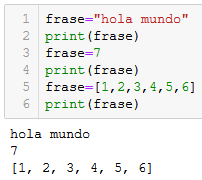
\includegraphics[width=0.4\textwidth]{img/unionesP.png}
\caption{Ejemplo de la flexibilidad de Python en cuanto a tipos}
\label{fig:unions1}
\end{figure}
\\

Diferencias entre lenguajes aparte, otra limitación viene dada por el propio parser, ya que no puede manejar declaraciones tipo \#define ver \ref{fig:define}
\begin{figure}[ht]
\centering
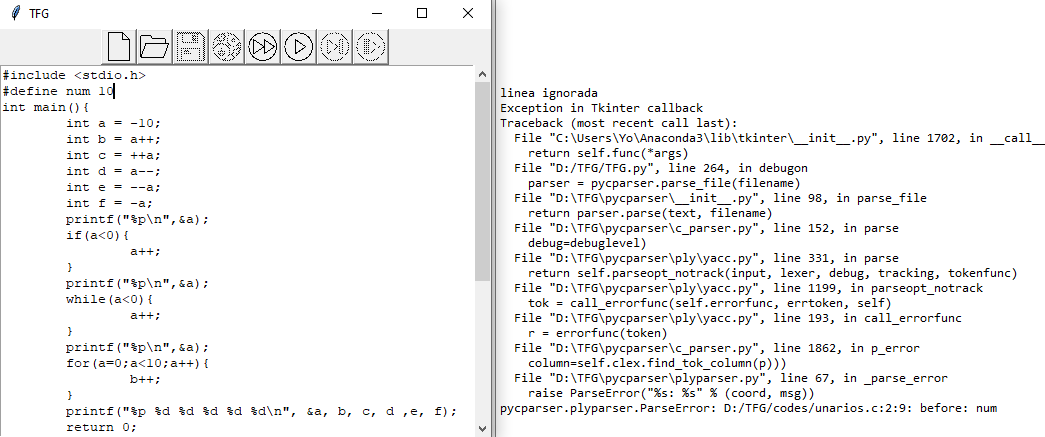
\includegraphics[width=\textwidth]{img/error_define.png}
\caption{Error al procesar los define}
\label{fig:define}
\end{figure}
\\

\section{Lineas de trabajo futuras}
\begin{itemize}
\item Una posibilidad sería añadir colorines de forma similar a lo que hacen el resto de asistenes o programas mas simples como sublime text o notepad++.
\item Otra posibilidad  es añadir más funciones propias de C, de momento el asistente solo incluye printf, scanf, strcpy, pow y sqrt.
\item Crear algún tipo de clase que permita la incorporación de las uniones y punteros.
\item Corrección de errores si se encontrasen.
\end{itemize}
